\chapter{基于多粒度切分的局部对齐网络}

\section{引言}
近年来,局部信息在计算机视觉的各种任务中发挥着越来越重要的作用,除了服装图像检索之外,这些任务还包括但不限于:细粒度分类、行人重识别、
视觉问答等。细粒度分类用于在一个大的类别中区分不同的小的类别,比如识别具体的鸟的品种,这需要着重对鸟的一些关键部位(比如嘴巴、眼睛)
做特征学习\cite{wang2018learning};类似的,行人重识别需要抽取行人特定部位(如头部、肩膀、腿部)的信息以消除因姿势不同带来的全局信息的偏差\cite{sun2018beyond};视觉问答任务里,
输入为一幅图像和与这幅图像相关的任何一个问题,算法需要输出这个问题的答案,需要对这幅图有全局的语义理解,同时根据问题侧重的学习相关的局部信息特征。
视觉问答的输入图像一般包括多个实例,输入问题有可能只关注其中的一部分,因此对局部信息的提取可以用目标检测框出所有的实例\cite{anderson2018bottom},而细粒度分类以及
图像检索任务一般涉及单个实例,需要采取不同的策略。

对单个实例的局部信息的学习一般有两种方式:基于软注意力(Soft attention)以及基于硬注意力(Hard attention)。软注意力指对图像不同区域的特征赋予不同大小的权重
,本文第三章提出的网络设计方式就是一种基于软注意力机制的方法,通过学习注意力权重分布图自适应的根据输入调节局部特征的权重以达到对局部信息的抓取,这种方法一般不需要
额外的标注信息去监督;硬注意力本质为软注意力机制的特征形式,软注意力的权重值是连续的(一般为0到1之间),而硬注意力机制则是0——1分布,即只保留部分局部区域的信息,
舍弃其余的信息。基于硬注意力机制的做法一般是通过对原图的切分来实现的,Wei等人提出一种基于关键点的切分方法\cite{wei2017glad},根据关键点所定位出的部件位置
生成检测框,随后再根据检测框对原图裁剪输入网络提取这部分的局部信息,这种方式有一定的有效性,但是需要依赖关键点的标注,对资源消耗较大。Li等提出一种无需额外标注
(只需要类别信息的标签)的切分方式\cite{li2017learning},其做法是直接对输入的图像横向平均切分,将每一个图像切片以及完整的原图送入网络做分类学习,且使用了不同大小的
卷积核对输入进行多尺度信息提取。

本章介绍一种具有创新性的基于切分的局部对齐网络结构,传统的基于切分去学习局部特征的做法大多数是对原图做切分,这种切分方式旨在通过对保留下的局部信息单独训练以达到增强
其语义强度的目的,但是这种直接舍弃大部分图像信息的方式不利于网络收敛,甚至会导致模型的过拟合,基于此弊端提出一种对特征图的切分方式。在此基础上对切分策略做了多方面的
改进,在强化局部特征语义信息的同时做到局部区域更好的对齐。
\section{方法与实现}
所提出的网络框架如图\ref{fig:MGN}所示,输入图像首先经过特征提取器提取特征,此处的特征提取器指基础网络(如ResNet)去除最后的全局池化层以及之后的部分,
输出的特征是一个张量,随后该特征复制若干份,并进入四个并行的分支:Global、Horizontal、Vertical、Annular。其中Global为全局分支,学习全局语义信息,
其余三个分支为局部分支,学习局部特征。
\begin{figure}[h]
  \centering
  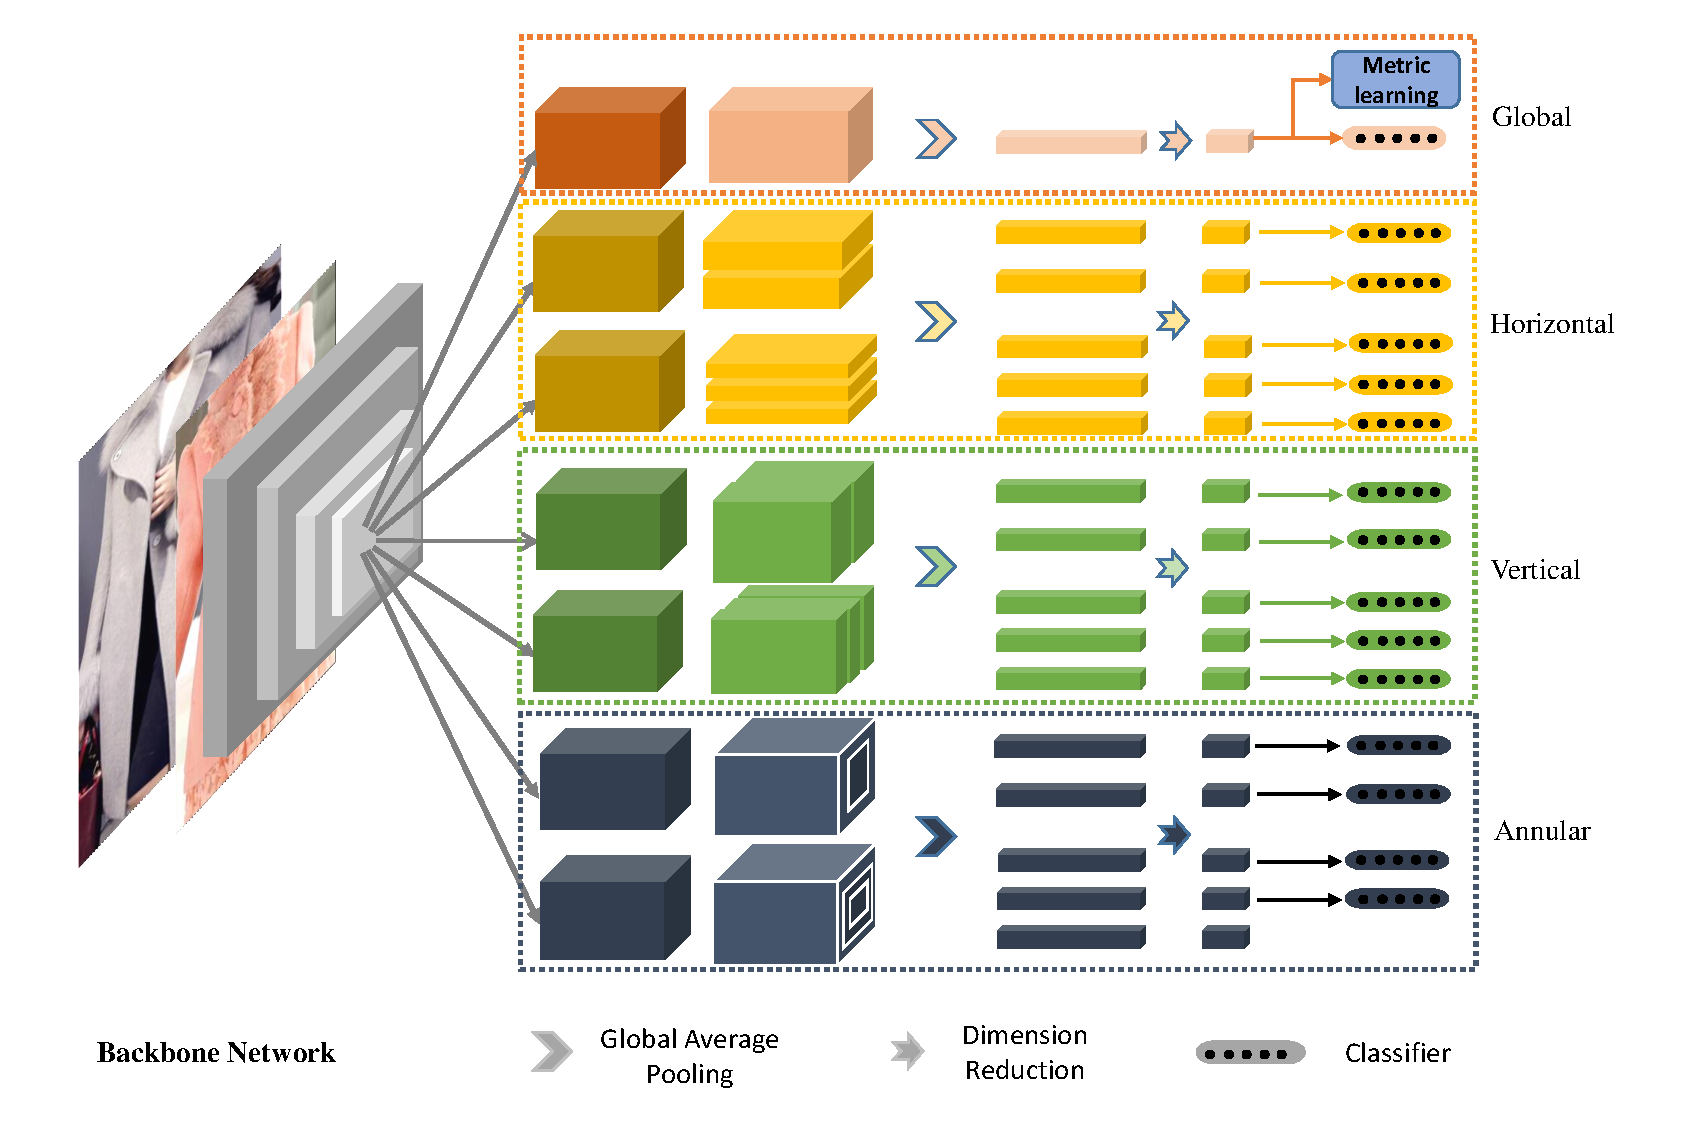
\includegraphics[width=1.0\linewidth]{Img/MGN.pdf}
  \caption{基于切分的局部对齐网络框架图}
  \label{fig:MGN}
\end{figure}

\subsection{对特征图的切分}
传统的基于切分的方式去学习局部特征的做法大多数是对原图做切分,然后将每个图像切片送入网络单独处理,而在本章所提出的方法中,切分操作是对特征图实施,如图\ref{fig:MGN}
中的局部分支所示。我们认为对原图切分之后保留的局部图像切片语义信息不够丰富,直接代表图像去识别其类别可能会导致过拟合,而基于特征图的切分则与之不同,
得益于卷积操作的特性,每个特征切片有着更丰富的上下文信息。
\begin{figure}[h]
  \centering
  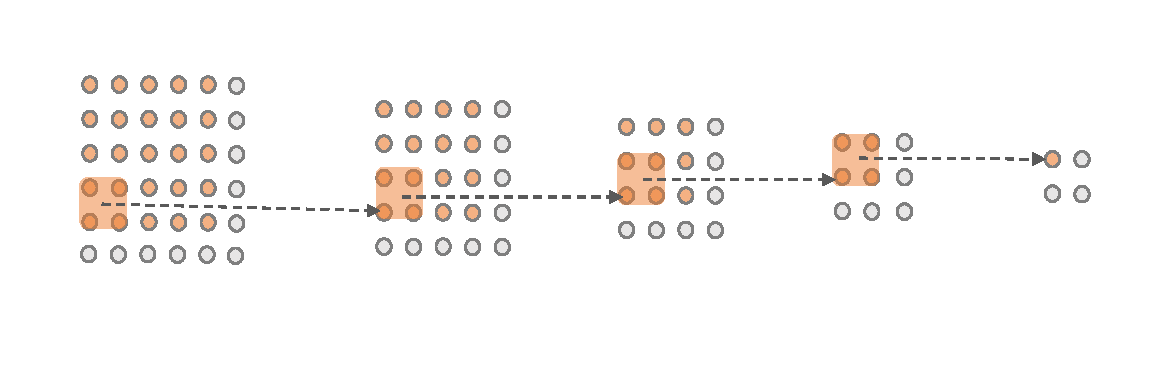
\includegraphics[width=1.0\linewidth]{Img/RF.pdf}
  \caption{卷积操作与感受野}
  \label{fig:RF}
\end{figure}


感受野(Receptive Field)是深度神经网络中的一个很常见的概念,它代表在特征图上的像素点映射到原图后的区域大小。而特征图上某个像素点的感受野的大小并不能按照原图和特征图大小的比例直接计算,
这是由卷积操作的特性所决定的,当前层的感受野与之前所有卷积层的参数都有关系。以图\ref{fig:RF}为例,假设输入图像大小为$6 \times 6$,经过四次卷积层,卷积核大小均为
$2 \times 2$,步长均为$1$,最后得到$2 \times 2$的输出,由图中感受野的变化情况可以看出:最后一层的输出特征图每个像素点对应的感受野对应原图的$5 \times 5$大小区域。

\begin{figure}[h]
  \centering
  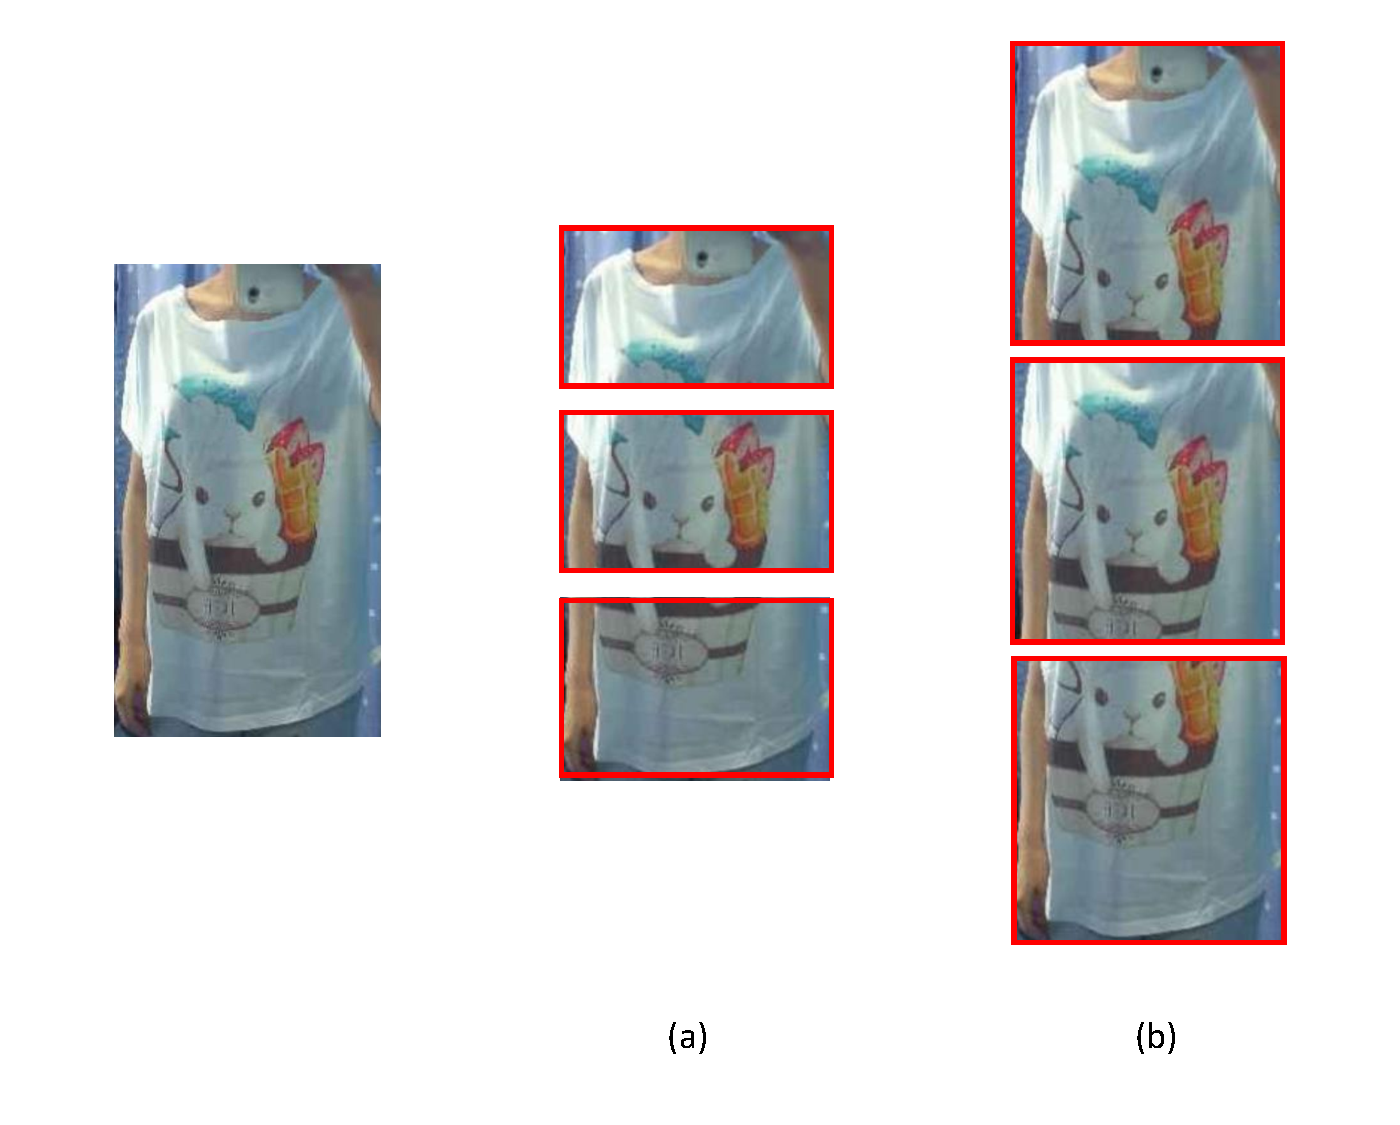
\includegraphics[width=0.8\linewidth]{Img/RFcmp.pdf}
  \caption{对原图切分和对特征切分的理论感受野差别}
  \label{fig:RFcmp}
\end{figure}

上述例子说明对特征图的切分和对原图的切分有根本区别,对特征图切分得到的特征切片包含了原图对应比例区域之外的上下文信息,如图\ref{fig:RFcmp}中,(a)、(b)分别代表
对原图和特征图切分后每个切片对应的理论感受野。然而,以(b)中所示感受野大小为准(有重叠区域)去切分原图和对特征图的切分仍然是不同的,
理论上来说,虽然特征图的每个切片对应的感受野比其在整个特征图所占比例在原图对应区域要大,但是这个区域的信息强度分布并不是平均的。Luo等人指出,卷积神经网络中的理论
感受野与实际感受野有很大差别,实际上来说越是靠近感受野中心的区域信号强度越大,整体呈高斯分布\cite{luo2016understanding}。因此,特征图的特征切片在包含更多的上下文
信息的同时,局部信息可以以相对更强的信号强度表达出来,而直接用有重叠区域的方式对原图切分反而会引入过强的噪音,导致不利于局部信息的表达。

我们对特征提取网络输出的张量进行切分,随后对每个切片进行全局平均池化得到若干向量,其维度为原特征图的通道数,然后用$1 \times 1$大小的卷积核对这个向量降维,
最后以降维后的向量作为局部特征的表示送入分类器学习原图的类别。分类器对应的损失函数就是Soft Max Loss,这么做的出发点是希望网络可以仅通过输入图像的某个局部区域去区分
其类别,这样可以提高局部区域特征的表达能力。所以,局部分支最后的特征由多个局部切片的向量组成:$\mathcal{F}=\{S_{1},S_{2}\cdots S_{i}\}$,
该分支的损失为$i$个Soft Max Loss的均值。
